\documentclass{scrartcl}

\usepackage[utf8]{inputenc}
\usepackage[T1]{fontenc}
\usepackage{lmodern}
\usepackage[ngerman]{babel}
\usepackage{amsmath}
\usepackage{hyperref}
\usepackage{pdfpages}



\usepackage{listings}
\lstset{numbers=left, numberstyle=\tiny, numbersep=5pt}
\lstset{language=Python}



% Default fixed font does not support bold face
\DeclareFixedFont{\ttb}{T1}{txtt}{bx}{n}{12} % for bold
\DeclareFixedFont{\ttm}{T1}{txtt}{m}{n}{12}  % for normal

% Custom colors
\usepackage{color}
\definecolor{deepblue}{rgb}{0,0,0.5}
\definecolor{deepred}{rgb}{0.6,0,0}
\definecolor{deepgreen}{rgb}{0,0.5,0}

\usepackage{listings}

% Python style for highlighting
\newcommand\pythonstyle{\lstset{
language=Python,
basicstyle=\ttm,
otherkeywords={self},             % Add keywords here
keywordstyle=\ttb\color{deepblue},
emph={MyClass,__init__},          % Custom highlighting
emphstyle=\ttb\color{deepred},    % Custom highlighting style
stringstyle=\color{deepgreen},
frame=tb,                         % Any extra options here
showstringspaces=false            % 
}}

% Python environment
\lstnewenvironment{python}[1][]
{
\pythonstyle
\lstset{#1}
}
{}




\begin{document}



\thispagestyle{empty}
\begin{center}
\Large{Hochschule Bochum}\\
\end{center}


\begin{center}
\Large{Fachbereich Elektrotechnik und Informatik}
\end{center}
\begin{verbatim}









\end{verbatim}
\begin{center}
\textbf{\LARGE{Dokumentation}}
\end{center}
\begin{verbatim}


\end{verbatim}
\begin{center}
\textbf{Softwareentwicklung mit NAO und ROS}
\end{center}
\begin{verbatim}














\end{verbatim}

\begin{flushleft}
\begin{tabular}{lll}

& & \\
& & \\
\textbf{eingereicht von:} & & Edgar Filipsen, Mika Katzwinkel, Jakob Kost,\\
 & &  Hubert Richter, Sebastian Schreiter\\
& & \\
& & \\
\textbf{eingereicht am:} & & 3. Februar 2017\\
& & \\
& & \\
\textbf{Betreuer:} & & Frau Prof. Dr. rer. nat. Brabender,\\
& & Dipl.-Ing. (FH) Andreas Koch
\end{tabular}
\end{flushleft}

\newpage
\tableofcontents
\newpage

\section{Einleitung}


\subsection{Projektbeschreibung}

Im Rahmen der Veranstaltung mussten wir uns, für die Bearbeitung von Softwareprojekten in Gruppen zusammenfinden. Anschließend musste sich jedes Team eine/n betreuende/n Professor/in suchen und mit dieser/m ein Projekt, zur Umsetzung innerhalb von 2 Semestern, planen und durchführen. Unser Team, bestehend aus Edgar Filipsen, Mika Katzwinkel, Jakob Kost, Hubert Richter und Sebastian Schreiter suchte sich Frau Prof. Dr. rer. nat. Brabender und Dipl.-Ing. (FH) Andreas Koch als Betreuer aus.
Da die Aufgabenstellung offen war, überlegten wir uns, dass der NAO Minigolf spielen soll. Dabei soll er Hindernisse selbstständig umspielen und schließlich ins Ziel treffen können.

\section{Eingesetzte Tools/Werkzeuge}

\subsection{ROS Indigo}
Bei dem Robot Operation System handelt es sich um ein Open Source Framework, welches für die Steuerung von Robotern eingesetzt werden kann. Die Hauptaufgaben von ROS sind Hardwareabstraktion, das Bereitstellen von Gerätetreibern, Paketverwaltung und der Nachrichtenaustausch zwischen Programmen bzw. Programmteilen. Das System ist aufgeteilt in das eigentliche Betriebssystem ros und ros-pkg, eine Auswahl an Zusatzpaketen, die das Basissystem um einzelne Fähigkeiten erweitern. Hierzu gehört zum Beispiel auch das Visualisierungstool RViz, welches wir verwendeten, um die Schlagbewegung des Roboters im Vorfeld zu simulieren. Außerdem finden sich dort auch einige Pakete für den NAO-Roboter, die wir in unsere Entwicklung mit einbringen konnten. Insgesamt gibt es mehr als 4000 zusätzliche Pakete, die größtenteils von der ROS-Community erstellt wurden. Dabei wird eine Serviceorientierte Architektur eingesetzt, um die Kommunikation zwischen den einzelnen Komponenten zu ermöglichen.

\subsection{Choreograph}
Choreograph ist die Standard Entwicklungsumgebung für den NAO Roboter, die, wie der Roboter selbst, auch von Aldebaran stammt. Hierbei wird die Programmierung über ein intuitives Drag- and Dropsystem realisiert, wodurch es auch Einsteigern leicht fällt, komplexere Abläufe zu programmieren. Wir nutzten in unserem Projekt Choreograph anfangs, um zum Beispiel das ''RedBall Tracking'' für unsere Zwecke zu testen. Hierbei war es auch besonders hilfreich, dass man sich den Python Code der einzelnen Funktionen anzeigen lassen kann. Später nutzten wir die Entwicklungsumgebung allerdings hauptsächlich nur noch für die Anzeige des Kamerabildes, um die Handlungen des Roboters besser nachvollziehen zu können.

\section{Eingesetzte Hardware}

\subsection{NAO Roboter}
Im ersten halben Jahr nutzten wir einen NAO Roboter, welcher uns freundlicherweise von Frau Dederichs-Koch des Fachbereichs M zur Verfügung gestellt wurde. Bei diesem traten leider des öfteren Probleme mit überhitzten Motoren und einem schwächelndem Akku auf.  
Mit dem NAO der neueren Generation traten diese weitaus seltener auf. Auch hat sich die Griffestigkeit der Finger stark verbessert.

Bei dem NAO handelt es sich um einen humanoiden Roboter der Herstellers Aldebaran.
Dieser ist etwa 60 cm groß und hat ein Gewicht von 5,2 kg. Er besitzt zwei Kameras, welche ihm eine Orientierung ermöglichen,  mehrere Mikrofone, Druck- und Berührungssensoren zur Interaktion, sowie ein Sonarsystem auf der Brust. Die Verbindung kann über Ethernet oder WLAN erfolgen. 



\subsection{Minigolf Ausrüstung}

\subsubsection{Die Bahn}
Da der neue NAO Schwierigkeiten mit dem Teppichboden unseres Büros hatte und um gleichbleibende Bedingungen zu ermöglichen, entschieden wir uns für eine Bahn aus Holz mit den Maßen: 2,5 m x 1,35 m. Bis auf den Startbereich ist die Bahn von einem 5 cm hohen Rand umgeben, welcher als Bande dienen soll. Das Ziel hat einen Durchmesser von 15 cm und ist 45 cm vom hinteren Rand entfernt (siehe Anhang A1). Zudem entschieden wir uns für zwei kreisrunde Hindernisse in blau und grün mit einem Durchmesser von 18 cm. Um  optimale Voraussetzungen für die Erkennung des Balls, sowie der Hindernisse zu ermöglichen wurde die Bahn weiß.

\subsubsection{Der Schläger}
Zu Beginn nutzten wir einen kleinen Minigolfschläger aus Plastik. Der NAO konnte diesen allerdings nicht  immer fest halten, besonders beim Ausholen und Schlagen verrutschte der Schläger in der Hand des NAOs. Daraufhin ließen wir von der mechanischen Werkstatt der Hochschule Bochum einen Schläger aus Aluminium mit einem zusätzlichen Griff anfertigen(siehe Anhang A2).

\subsubsection{Der Ball}
Wir testeten über Monate verschiedene Bälle, sowohl in Hinblick auf Größe als auch auf Material. Die Wahl der Farbe fiel direkt auf rot, da der NAO bereits eine "Redball Detection" besitzt. Wir entschieden uns für einen massiven Gummiball mit einem Durchmesser von 6 cm.  


\section{Installation}


\subsection{Installation von ROS}

Für das Projekt entschieden wir uns für ROS Indigo, die aktuellste Version mit Langzeitunterstützung.
Die Installation erfolgte auf Ubuntu 14.04 
Als Grundlage nutzten wir das offizielle Installationstutorial des ROS Wikis.
Zunächst mussten Pakete von packages.ros.org akzeptiert werden. Der Befehl dazu lautet: 
\begin{align}
&sudo\ sh\ -c\ 'echo\ ``deb\ http://packages.ros.org/ros/ubuntu \\ 
&\$(lsb\_release\ -sc)\ main"\ >\ /etc/apt/sources.list.d/ros-latest.list'
\end{align}
Außerdem muss noch die Schlüssel ID  zur Authentifizierung der Pakete vom Server heruntergeladen werden:
\begin{align}
&sudo\ apt-key\ adv\ --keyserver\ hkp://ha.pool.sks-keyservers.net\\ 
& --recv-key\ 0xB01FA116
\end{align}
Mit dem Befehl 
\begin{align}
&sudo\ apt-get\ install\ ros-indigo-desktop-full
\end{align}
wird die komplette Installation gestartet, die folgende Komponenten enthält: ROS, rqt, rviz, robot-generic libraries, 2D/3D Simulatoren, Navigation und Pakete für die 2D und 3D Wahrnehmung.
\\
Bevor ROS nun genutzt werden kann, muss rosdep initialisiert werden. Dies erlaubt die einfache Eingabe von...
\begin{align}
&sudo\ rosdep\ init\\
&rosdep\ update
\end{align}
Um die setup.bash Datei nicht bei jedem Öffnen einer neuen Shell sourcen zu müssen, empfiehlt es sich, diesen Befehl in die .bashrc-Datei zu kopieren.
Dafür nutzten wir folgende Befehle:
\begin{align}
&echo\ ``source\ /opt/ros/indigo/setup.bash"\ >>\ \sim/.bashrc\\
&source\ \sim/.bashrc
\end{align}

\subsection{Erstellen eines Workspaces}

Nach der Installation ist es nötig, einen Workspace zu erstellen, in dem gearbeitet wird.

\begin{align}
&\$\ mkdir\ -p\ \sim/catkin\_ws/src\\
&\$\ cd\ \sim/catkin\_ws/src\\
&\$\ catkin\_init\_workspace
\end{align}

\subsection{Tutorial}

Auf der ROS-Wikiseite
\url{http://wiki.ros.org/ROS/Tutorials} finden sich viele Tutorials, welche den Umgang mit dem ROS Filesystem, Packages und Nodes, sowie das Schreiben von Publishern und Subscribern in C++ oder Python beschreiben.
Diese wurden von uns zur Einarbeitung bearbeitet.

\subsection{Installation von RVIZ}

Die Installation von RViz war bereits im Installationspaket von ROS enthalten und musste hierfür nicht noch einmal gesondert installiert werden. Allerdings musste noch zusätzlich das ganze NAO-Paket, wie z.B. Treiber u.Ä. installiert werden. Über die Seite 
\url{http://wiki.ros.org/nao/Tutorials/Installation}  gelangt man zu einem Tutorial, in dem alles Nötige erklärt wird. Nachdem wir dieses Tutorial durchgearbeitet hatten, war die Installation aller wichtigen Komponenten fast fertiggestellt. Um ein schon fertiges Modell des NAO-Roboters benutzen zu können, mussten wir noch ein zusätzliches Paket herunterladen und dazu einer Lizenzbestimmung zustimmen. Dieses wird über den Befehl
\begin{align}
&sudo\ apt-get\ install\ ros-indigo-nao-meshes
\end{align}
heruntergeladen und installiert.

\subsection{Konfiguration von RVIZ für den NAO}

Bei der Konfiguration von ROS für den NAO-Roboter sahen wir uns einigen Problemen gegenübergestellt. Zunächst war das Tutorial, welches auf der ROS-Wikiseite zu finden ist, veraltet. Das Problem dabei war, dass dieses das einzige Tutorial war, das wir auffinden konnten. Deshalb mussten wir uns erst einmal eine ganze Weile mit RViz auseinander setzen. Nach dem Durchforsten einiger Foreneinträge und auch ein wenig Ausprobieren, fanden wir dann die richtigen Befehle, um eine ordentliche Simulation des NAO über RViz laufen zu lassen.
Zunächst wird der Roscore gestartet:
\begin{align}
&cd\ \sim/catkin\_ws\\
&roscore
\end{align}
Anschließend werden die Simulation und die dazugehörigen Treiber gestartet:
\begin{align}
&\sim/naoqi/naoqi\-sdk\-2.1.4.13\-linux64/naoqi\ --verbose\ \-\-broker-ip\ 127.0.0.1\\
&roslaunch\ naoqi\_driver\_py\ naoqi\_driver.launch
\end{align}
Für den letzten Schritt bearbeiteten wir eine bereits vorhandene .launch-Datei so, dass RViz nach unseren Vorstellungen das Modell lädt. Das ganze startet man dann über folgenden Befehl:
\begin{align}
&roslaunch\ nao\_description\ display.launch
\end{align}
display.launch ist hierbei unsere editierte Datei.
Damit haben wir einen simulierten NAO-Roboter, dem wir per Konsole Befehle erteilen können.

\subsection{Einarbeitung in NAO-API}

Nachdem wir dem NAO-Roboter ein paar Befehle direkt über die Konsole erteilt hatten, ging es nun darum, ihn komplexere Befehlssätze ausführen zu lassen. 
Dazu mussten wir uns allerdings zunächst in die NAO-API einarbeiten, welche unter folgender Adresse zu erreichen ist:\\
\url{http://doc.aldebaran.com/1-14/naoqi/index.html} \\
Zusätzlich dazu schauten wir uns auch einige Code-Beispiele zu wichtigen Themen, wie z.B. der Ballerkennung an, um die Funktionsweise der einzelnen Befehle zu verstehen.


\section{Programmierung}


\subsection{Erste Schritte}

Nachdem wir die Installation und Konfiguration durchgeführt hatten, testeten wir zunächst einige Grundfunktionen anhand der Visualisierung mit RViz.
Hierbei nutzten wir die Konsole um Befehle direkt zu übermitteln. Dabei stellten wir fest, dass einige Befehle in der Visualisierung nicht umgesetzt werden konnten, da das genutzte Modell in RViz nicht vollständig war.
Im Anschluss führten wir die Kommandos am Roboter aus, was weniger Probleme verursachte, als wir uns vorgestellt hatten. 
Dennoch mussten wir uns noch viel mit der NAO-API auseinander setzen, um die benötigten Schnittstellen zu finden.

Mit dem Befehl
\begin{align}
rosrun rviz rviz
\end{align}

wird RViz gestartet und mit 

\begin{align}
&rostopic pub -1 /cmd\_vel geometry\_msgs/Twist\\ &'{linear: {x: 1.0, y: 0.0, z: 0.0},angular: {x: 0.0, y: 0.0, z: 0.0}}'
\end{align}
beginnt der virtuelle NAO sich vorwärts zu bewegen. Die linearen Variabeln geben die Richtung, angular die ???? an.

\subsection{Schlagbewegung}

Um die Schlagbewegung durchzuführen testeten wir zunächst die ungefähren Bewegungen in der Simulation. Am Roboter führten wir danach die Feinabstimmung durch und nutzten dabei einen kleinen Spielzeuggolfschläger. 
Da sich in diesem Abschnitt herausstellte, dass das Ausführen unter ROS sehr viel Zeit beanspruchte, verzichteten wir im Folgenden temporär auf ROS und nutzten stattdessen einfache Python-Skripte, um Änderungen schneller austesten zu können.
Die Funktion angleInterpolation nimmt 4 Parameter entgegen. Der erste ist ein Array von Gelenken die bewegt werden sollen. Jedes Gelenk hat einen Bereich in dem es bewegt werden kann, die Punkte dieser Bereiche die angesteuert werden sollen, werden in einem Array als zweiter Parameter übergeben. Im dritten Array wird für jedes Gelenk eine Zeit in Sekunden angeben in der die gewünschte Position erreicht werden soll. Der letzte Parameter ist ein boolscher Wert, 0 gibt an dass die Bewegung relativ zur vorherigen Position ist, bei 1 wird eine absolute Position angesteuert.

\begin{python}

# Golf Swing Motion
def hit():
    motion.angleInterpolation(["RShoulderRoll","RShoulderPitch",
       "RElbowRoll","RElbowYaw","RWristYaw"],
       [[0.3],[1.2],[1.2],[1.65],[-0.15]],
       [[1.0],[1.0],[1.0],[1.0],[1.0]],1)
    motion.angleInterpolation(["RShoulderRoll","RShoulderPitch",
       "RElbowRoll","RElbowYaw","RWristYaw"],
       [[0.3],[1.2],[1.2],[1.65],[-0.9]],
       [[1.0],[1.0],[1.0],[1.0],[1.0]],1)

    time.sleep(2)

    motion.angleInterpolation(["RWristYaw"],[0.4],[0.75],1)
    motion.angleInterpolation(["HeadYaw","HeadPitch"],
    	[[1.0],[0.5]],[[1.0],[1.0]],1)

    time.sleep(3)
    say("hit")

    motion.angleInterpolation(["HeadYaw","HeadPitch"],
    	[[0],[0]],[[1.0],[1.0]],1)
\end{python}

\subsection{Ballerkennung}

Da der NAO bereits eine Funktion für die Erkennung eines roten Balls besitzt, nutzten wir diese direkt. Hierfür besorgten wir uns einen roten Plastikball und führten erste Versuche durch, um die Funktion für unsere Zwecke einsetzen zu können.
Allerdings mussten wir hierbei einige Anpassungen vornehmen, weil die Kamera des NAO nur einen bestimmten Sichtbereich hat und der Bereich direkt vor dem Roboter nicht mehr sichtbar ist. Da wir deshalb das letzte Stück ''blind'' steuern mussten, kam es hierbei auch häufig zu Ungenauigkeiten beim Schlag. Daraus resultierte eine schwer zu kalkulierende Ballbewegung, für die wir auch erstmal keine Lösung fanden. Wir nahmen uns vor, diese Problemstellung zu einem späteren Zeitpunkt noch einmal zu bearbeiten und uns zunächst mal um die Erkennung des Zieles zu kümmern. Letztendlich wurde die Bewegung die die Lücke überbrückt so angepasst, dass der Unterschied der Entfernungen zum Ball bei verschiedenen Anläufen so klein ist, dass er zu vernachlässigen ist. 

\begin{python}
def trackBall():
    lookDown()
    # Add target to track
    targetName = "RedBall"
    diameterOfBall = 0.06
    tracker.registerTarget(targetName, diameterOfBall)

    # Set mode
    mode = "Move"
    tracker.setMode(mode)
    tracker.setMaximumDistanceDetection(3.0)
    tracker.setRelativePosition([-0.55,0,0,0.01,0.01,0.01])

    tracker.setMoveConfig([["Frequency",0.005]])
    # Start tracker
    tracker.track(targetName)

    global targetReached
    while(not targetReached):
        time.sleep(1)
    targetReached = False
    
# Module for Balltracking
class TrackerModule(ALModule):
    def __init__(self, name):
        ALModule.__init__(self, name)

        memory.subscribeToEvent("ALTracker/TargetReached",
            "Tracker",
            "onTargetReached")

    def onTargetReached(self, *_args):
        print "Target reached"
        tracker.stopTracker()
        tracker.unregisterAllTargets()
        #Walk remaining distance to ball
        motion.moveTo(0.27,0.03,0,
            [["MaxStepFrequency",0.01],["MaxStepX",0.025]])
        global targetReached
        targetReached = True
    
\end{python}

\subsection{Zielen}

Um auf das Ziel und um Hindernisse herum zu spielen, nahmen wir uns eine Funktion des NAOs zu Hilfe, die anhand eines farbigen Kreises die Koordinaten dieses Kreises ermittelt. Das Koordinatensystem bezieht sich hierbei auf den Sichtbereich des Roboters. Die X-Achse  
hat einen Bereich von 0-160, die Y-Achse von 0-120, der Nullpunkt liegt oben links. Da das Kamerabild vom NAO kommt, liegt sein Referenzpunkt unten in der Mitte, also bei (80,120). Hat man nun diese zwei Punkte gegeben, lässt sich ein Dreieck bilden, dessen Hypotenuse die Verbindung zwischen NAO und Ziel darstellt. Da sich alle Längen des Dreiecks mithilfe der Längen der Achsen und den Koordinaten der Punkte errechnen lassen, kann auch der Winkel zwischen NAO und diesem Ziel berechnet werden. Nun musste nur noch eine Kreisbewegung programmiert werden, die den Roboter gleichmäßig um den Ball führt. Schließlich kann durch Messungen der Drehdauer eine Funktion bestimmt werden, die anhand eines Winkels die Zeit zurückgibt, die benötigt wird, damit der Roboter sich um diesen Winkel dreht.\\


\begin{python}
def turnToTarget(target):

    # Calculate angle to Target
    if(target[0] <= 80):
        degree = math.degrees(math.atan(
        	(120-target[1])/(80-target[0])))
    else:
        degree = 90 + math.degrees(math.atan(
        (target[0]-80)/(120-target[1])))

    # Calculate time to turn
    global turnTime
    turnTime = 0.079318*degree + 7.901573

    # Turn
    motion.move(0,0.02,-0.084)
    time.sleep(turnTime)
    motion.move(0,0,0)
\end{python}
 
\subsection{Erkennen der Hindernisse}

Für die Erkennung der Hindernisse nutzen wir die selbe Methode wie für die Zielerkennung. Für die Ermittlung der Positionen wurde die Bahn in drei Abschnitte geteilt: rechts, mitte und links.  Da sich das Sichtfeld des NAOs wie beim Menschen auch nach hinten hin verzerrt, musste zunächst eine Funktion zur Ermittlung der Abschnitte erstellt werden. Dabei wird je nach Entfernung eines Hindernisses die jeweilige Bahnbreite in Pixeln bestimmt.
Diese wird dann durch drei geteilt um die Bahn in die entsprechenden Bereiche einzuteilen. Somit kann erkannt werden in welchen Bereichen sich die Hindernisse befinden und somit eine Entscheidung getroffen, in welche Richtung gespielt werden soll. Mit Hilfe der Zielfunktion wird dann je nach Aufstellung gegen die Bande auf Höhe eines Hindernisses oder geradeaus durch die Mitte geschlagen.

\begin{python}
#Get half of coursewidth
def getWidth(height):
    return 1.171484*height+7.923894 

def aim():
    print "aim"
    global gr1
    global gl1
    global gr2
    global gl2

    gr1 = 80 + getWidth(oc1[1]/3)
    gl1 = 80 - getWidth(oc1[1]/3)
    gr2 = 80 + getWidth(oc2[1]/3)
    gl2 = 80 - getWidth(oc2[1]/3)

    if((oc1[0]<gl1 or oc1[0]>gr1) and 
    	(oc2[0]<gl2 or oc2[0]>gr2)):
           # play straight
           turnToTarget([58.5,20])
    elif(oc1[0]<gl1 and oc2[0]>=gl2 and oc2[0]<=gr2):
           # play right to obstacle 2
           turnToTarget([80+getWidth(oc2[1]),oc2[1]])
    elif(oc1[0]>gr1 and oc2[0]>=gl2 and oc2[0]<=gr2):
           # play left to obstacle 2
           turnToTarget([80-getWidth(oc2[1]),oc2[1]])
    elif(oc1[0]>=gl1 and oc1[0]<=gr1 and oc2[0]<gl2):
           # play right to obstacle 1
           turnToTarget([80+getWidth(oc1[1]),oc1[1]])
    elif(oc1[0]>=gl1 and oc1[0]<=gr1 and oc2[0]>gr2):
           # play left to obstacle 1
           turnToTarget([80-getWidth(oc1[1]),oc1[1]])
    else:
           # play left to both obstacles
           mid = (oc1[1] + oc2[1]) / 2
           turnToTarget([80-getWidth(mid),mid])

    time.sleep(2)
    takeClub()
    hit()
    giveClub()
    turn(turnTime,"anticlockwise")
    checkObstacles()

\end{python}

\subsection{Weiterer Spielverlauf}

Nach dem ersten Schlag bewegt sich der Roboter zunächst zurück in seine Ausgangsposition um den Ball zu lokalisieren. Danach wird überprüft ob der Ball an einem oder beiden Hindernissen vorbei gespielt wurde und ob er hinter einem Hindernis liegt oder nicht. Dementsprechend werden verschiedene Laufbewegungen ausgeführt, die den Roboter um die Hindernisse herum und zum Ball führen. Diese bestehen zum einen Teil aus dem automatischen RedBallTracker und zum anderen Teil aus manuellen Bewegungen. Gegebenenfalls wird erneut um ein Hindernis herum gespielt und gelaufen. Sobald dem Ziel nichts mehr im Weg steht wird mithilfe der Zielfunktion auf dieses gespielt. Nach dem Schlag wird überprüft ob der Ball noch zu sehen ist. Sollte dies der Fall sein, was bedeutet, dass verfehlt wurde, so wird das Spiel als verloren angesehen. Wenn der Ball sich im Loch befindet und nicht mehr zu sehen ist, ist die Aufgabe erfüllt. Dem Ergebnis entsprechend wird eine passende Audioausgabe abgespielt und das Programm beendet.  

\begin{python}
# Module after first shot
class ObstacleModule2(ALModule):
    def __init__(self,name):
        ALModule.__init__(self,name)

    def onBlobDetected(self,*_args):
        memory.unsubscribeToEvent("ALTracker/ColorBlobDetected",
        	"Obstacle2")
        global oc1
        global oc2
        global bc

        searchBall()
        
        if(oc1[1]>bc[1]):
            print "hindernis 1 naeher als ball"
            if(oc2[1]>bc[1]):
                print "ball hinter hindernissen"
                walkBetweenTargets(oc1,oc2)
                avoidSecondObstacle()
                searchGoal()
                playGoal()
            else:
                walkToBallBetweenTargets(oc1,oc2)
        else:
            print "ball naeher als hindernisse"
            

\end{python} 

Hätte der Ball beispielsweise nach dem ersten Schlag beide Hindernisse überwunden, würde der Roboter zunächst das erste Hindernis umlaufen, danach das zweite und schließlich das Ziel suchen und darauf zielen.

Die nachfolgende Funktion zeigt, wie ein Hindernis umlaufen wird falls der Ball nicht dahinter liegt. In diesem Fall wird zunächst seitlich auf die Höhe des Balls gelaufen und dann der RedBallTracker eingesetzt um bis zum Ball zu laufen.

Anhand der Entfernung des Balls wird zunächst die Bahnbreite auf dieser Höhe berechnet. Mithilfe der Koordinaten des Balls wird die prozentuale Entfernung des Balls von der Mitte in Abhängigkeit von der Bahnbreite ermittelt. Durch den Prozentsatz wird eine Zeit bestimmt, die der Roboter seitlich läuft.


\begin{python}
# Ball not behind obstacle
def walkToBall():
    print "walkToBall"
    width = getWidth(bc[1])
    global sec
    global pos
    if(bc[0]>80):
        pos = 1
        ballPixel = bc[0] - 80
        percent = ballPixel/width
        sec = 20*percent
        moveSideways(sec,"right")

    else:
        pos = 2
        ballPixel = 80 - bc[0]
        percent = ballPixel/width
        sec = 20*percent
        moveSideways(sec,"left")

    trackBall()
\end{python}


\subsection{Entwicklung mit ROS}
Da wir, wie oben bereits genannt, zur Entwicklung hauptsächlich ein einfaches Python Skript verwendeten, entschieden wir uns, nach Absprache mit Frau Brabender, dazu, die Entwicklung mit und ohne ROS separat zu behandeln, um die Unterschiede in der Handhabung darstellen zu können. Dabei wurde deutlich, dass die Integration des Codes in ROS schneller erledigt war, als erwartet und doch einige Möglichkeiten bietet. Ein grundlegender Unterschied bei der Integration von ROS war die Implementierung der Node Struktur von ROS. Hierbei werden die Funktionen in einer Node Klasse zusammengefasst, die als Objekt über ROS initialisiert werden kann. Sobald dieses dann erstellt wurde, dient es sozusagen als Grundstruktur für die Funktionalitäten und wird über ROS aufrecht erhalten. Anschließend kann dann über diverse ROS eigene Befehle auf die erstellten Dienste, Sender, Empfänger etc. zugegriffen werden. Außerdem hat man auch jederzeit eine gute Übersicht über die gesamte Struktur der unterschiedlichen Nodes und ihrer verfügbaren Dienste und kann sich diese sogar graphisch darstellen lassen.
Bei der Integration war besonders darauf zu achten, dass die Node Klasse bereits einen Broker, welcher die Verbindung zum Roboter aufbaut, enthält, welcher nur noch mit IP und Port des Roboters gefüllt werden muss. Somit erübrigte sich auch die Erstellung eines separaten Brokers, wie vor der Integration.
Als Ergebnis lässt sich zusammenfassen, dass die Integration von ROS einen sehr guten Überblick über die vorhandenen Funktionalitäten bietet und gerade bei unübersichtlichen, großen Projekten die Arbeit deutlich erleichtern kann. Zusätzlich wird auch eine einheitliche Struktur eingeführt, die auch bei der Arbeit mit anderen Robotern immer gleich bleibt. Bei unserem Projekt hatte die Integration von ROS allerdings wenig Einfluss, da das Projekt keinen so großen Umfang hatte und die Struktur von ROS hier kaum zum Einsatz kommen konnte.

\newpage
\appendix 


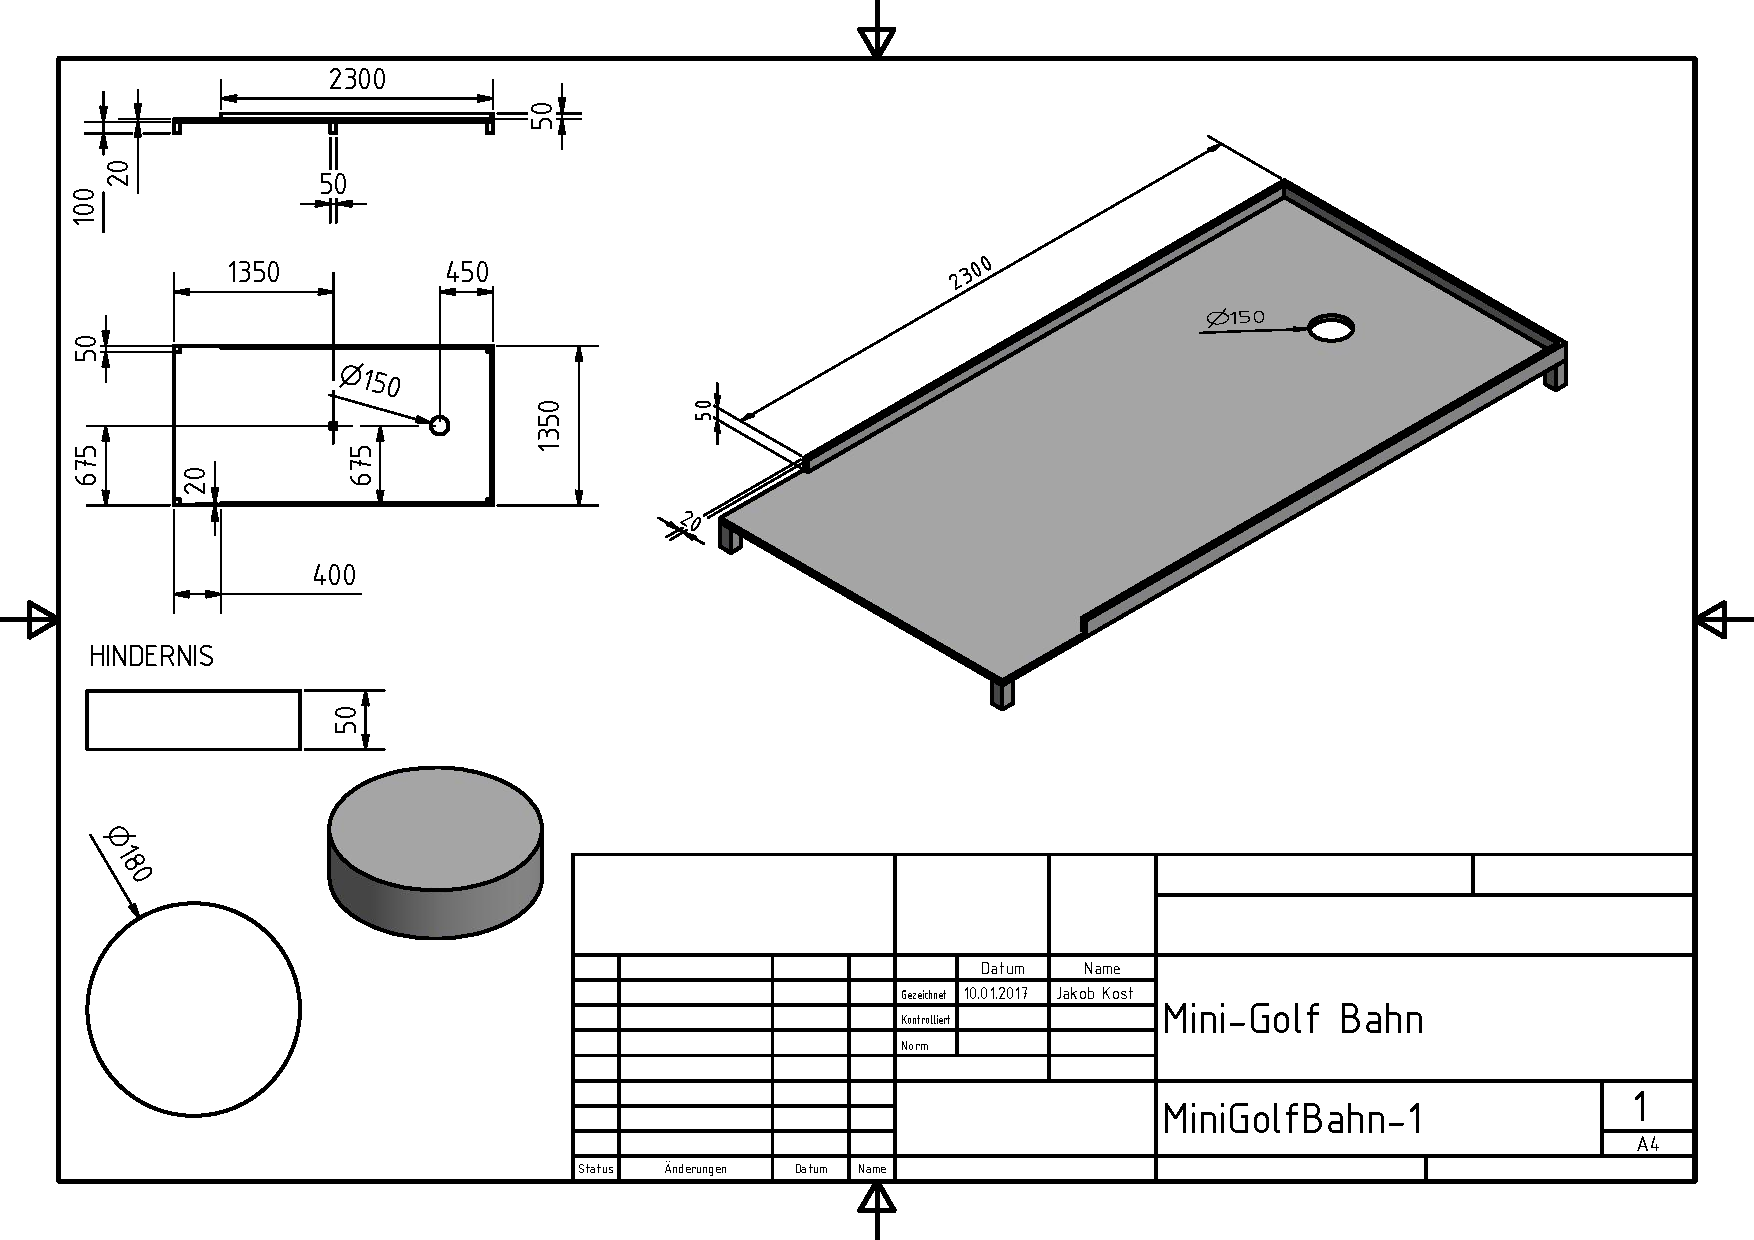
\includepdf[pages=1,pagecommand=\section{Anhang}\subsection{Minigolfbahn }]{MiniGolfBahn.pdf} 

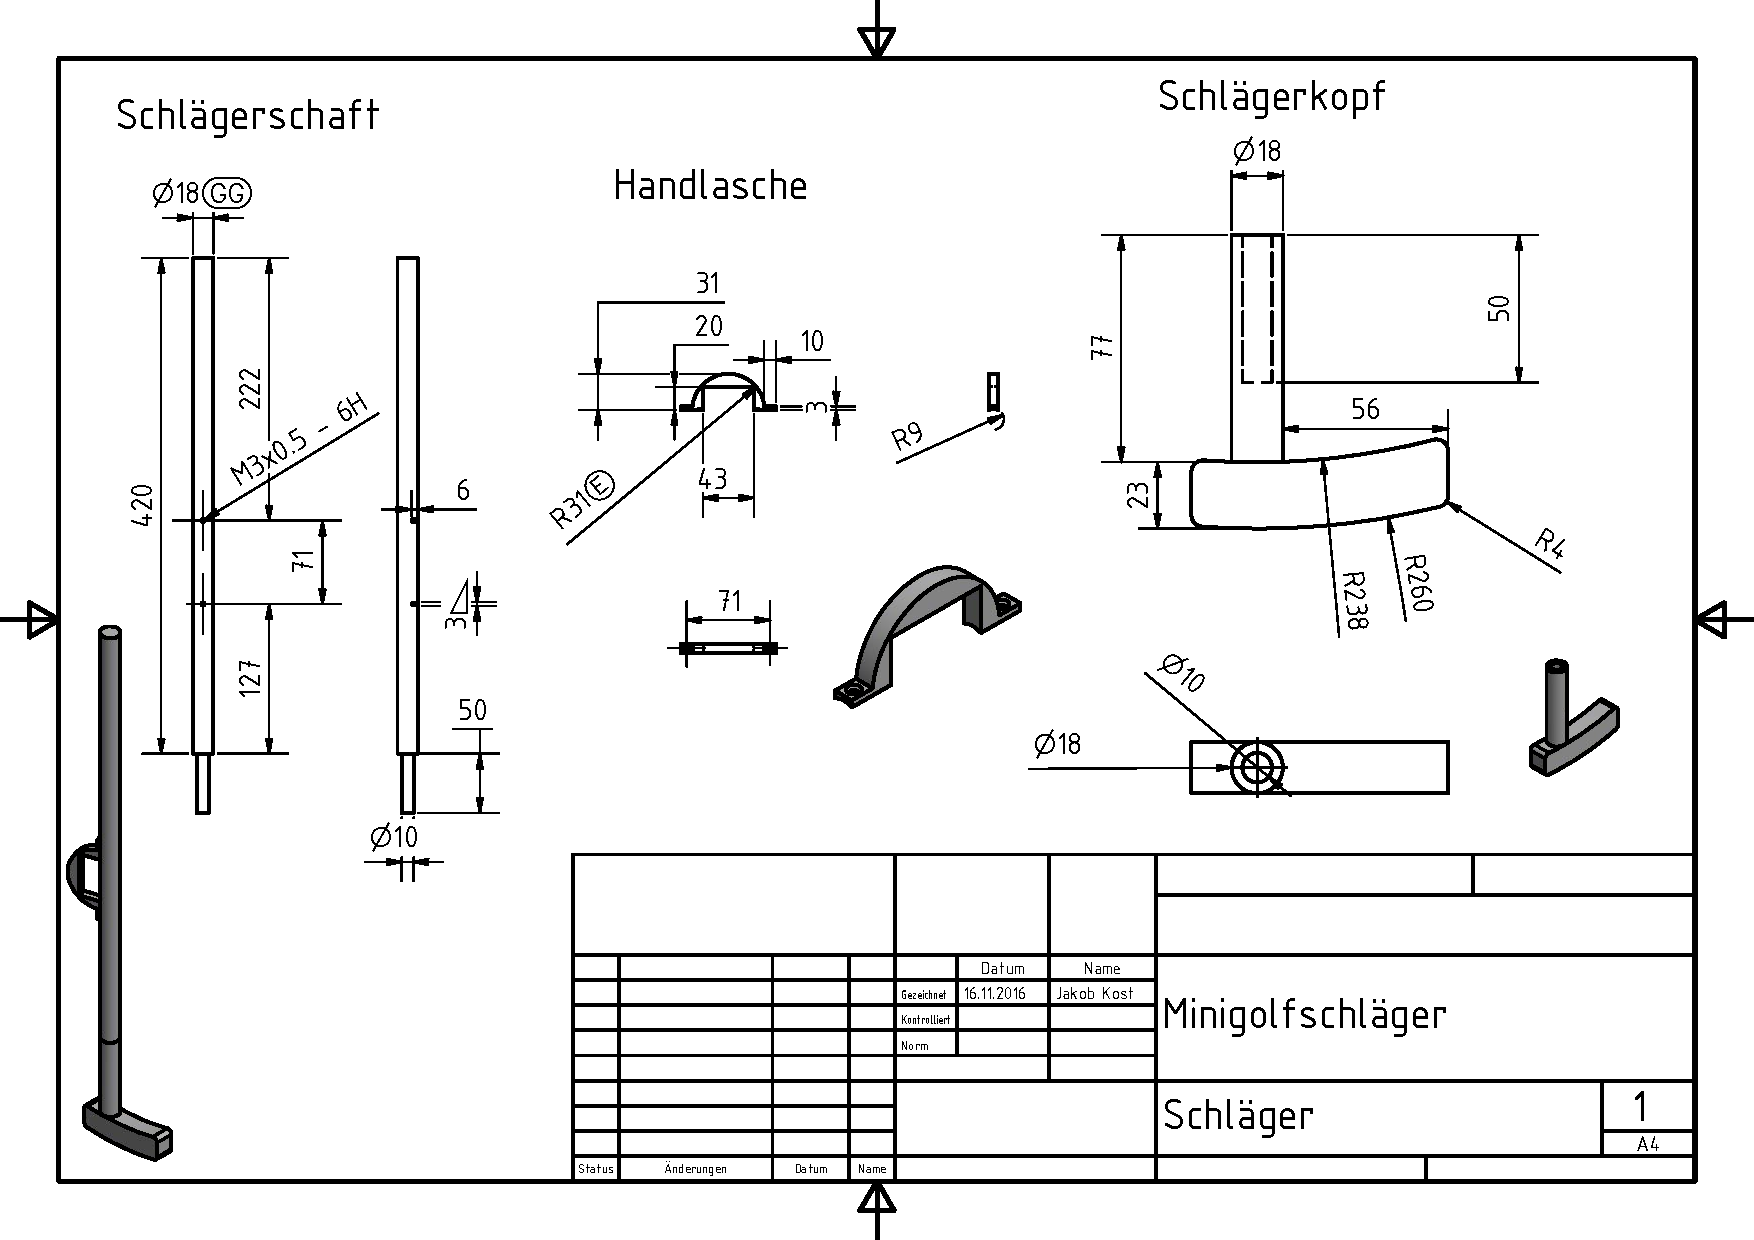
\includepdf[pages=1,pagecommand=\subsection{Schläger }]{Schlaeger.pdf} 
 

\end{document}
